\chapter{Evaluasi}

%=============================
\section{ABS MVC Framework}
%=============================
ABS MVC Framework merupakan sebuah web application framework berbasis Model-View-Controller (MVC) yang dibangun dengan menggunakan bahasa pemodelan ABS. Tujuan dibangunnya framework ini adalah untuk membantu para pengembang perangkat lunak untuk memanfaatkan bahasa pemodelan ABS dalam menghasilkan sebuah perangkat lunak berbasis web. Selain itu, framework ini juga dapat membantu para pengembang perangkat lunak untuk dapat menerapkan pola MVC dalam proses pengembangan aplikasi web yang mereka lakukan. Penerapan pola MVC tersebut nantinya akan membantu para pengembang perangkat lunak dalam memisahkan logika aplikasi, data dan presentasi dari setiap berkas kode yang dibuat sehingga akan meningkatkan \textit{maintainability} dari perangkat lunak yang dihasilkan.

\subsection{Arsitektur Framework}
Framework MVC ABS dibangun atas tiga bagian yang diantaranya adalah:
\begin{itemize}
    \item \textbf{HTTP Helper}: merupakan komponen framework yang bertugas untuk menangkap HTTP Request dan memberikan HTTP Response kepada web server. Komponen ini dibuat dengan menggunakan bahasa pemodelan ABS.
    \item \textbf{URL Router}: merupakan komponen framework yang bertugas untuk melakukan pemetaan terhadap setiap URL request yang diterima dari web server kedalam application Controller yang dibuat. komponen ini juga dibuat dengan menggunakan bahasa pemodelan ABS.
    \item \textbf{Application Builder}: merupakan komponen framework yang bertugas untuk melakukan proses kompilasi kode program dan membungkusnya kedalam bentuk JAVA Archive (jar) untuk kemudian di \textit{deploy} ke dalam web server. komponen ini dibuat dengan menggunakan Apache Ant.
\end{itemize}

\noindent
komponen-komponen framework di atas berperan dalam membantu para pengembang perangkat lunak untuk dapat menghasilkan sebuah perangkat lunak berbasis web dengan menggunakan bahasa pemodelan ABS.

\subsection{Struktur Direktori}
Struktur direkretori dalam sebuah framework MVC berperan dalam membantu para pengguna framework untuk mengatur peletakan setiap kode program yang mereka hasilkan sesuai dengan kategori / jenis dari kode program tersebut. Dengan adanya struktur direktori yang baik, akan membantu para pengembang perangkat lunak untuk dapat konsisten dalam meletakkan setiap kode program yang mereka hasilkan. berikut ini adalah struktur direktori dari framework MVC ABS:

\begin{itemize}
    \item \textbf{dist}: folder ini digunakan untuk menyimpan binary dari aplikasi web yang sudah di compile.
    \item \textbf{src}: folder ini digunakan untuk menyimpan file ABS yang dibuat oleh para pengembang perangkat lunak. folder ini memiliki sub folder "Model", "View" dan "Controller" yang digunakan untuk meletakkan komponen MVC yang dibuat. Selain itu, di dalam folder ini juga terdapat sebuah folder bernama "Framework" yang berisi berkas kode program ABS yang digunakan untuk keperluan internal framework.
    \item \textbf{lib}: folder ini berisi library yang dibutuhkan oleh framework MVC ABS untuk dapat meng-compile kode ABS dan mengubahnya ke dalam kode JAVA.
    \item \textbf{target}: folder ini digunakan sebagai tempat penampungan sementara ketika framework sedang melakukan proses kompilasi kode ABS.
\end{itemize}

\begin{figure}
    \centering
    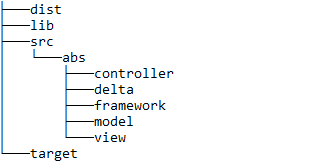
\includegraphics[width=0.8\textwidth]
        {img/struktur-direktori.png}
    \caption{Struktur Direktori ABS MVC Framework}
\end{figure}

\subsection{Cara Kerja Framework}


%=============================
\section{ABS MVC Server}
%=============================